%%
% La siguiente plantilla esta basada en el siguiente enlace:
% http://academic.reed.edu/physics/courses/Physics332.s08/reports.html
% La plantilla original puede descargarse de ese sitio
% Se dejo parte del texto original en inglés para ilustar el uso de la plantilla
% Se hicieron algunas modificaciones para ajustar el idioma y otros detalles para 
% completar un reporte técnico breve pero muy puntual
% Modificación Inicial: Marco Aurelio Nuno Maganda - 11/SEP/2014
% 
% Enlace a la documentación del tipo de documento base (revtex4)
% http://mirror.hmc.edu/ctan/macros/latex/contrib/revtex/doc/latex/revtex/source/revtex4-1.pdf
%
% En algunas distribuciones es necesario instalar el paquete texlive-publishers
%
%\documentclass[letterpaper,aps,twocolumn,pre,nofootinbib]{revtex4}
%\documentclass[twocolumn]{article}
\documentclass[conference]{IEEEtran}

\usepackage[spanish]{babel}
\usepackage{amsmath,amssymb,amsfonts,amsthm}
\usepackage{graphicx}
%\usepackage{bbm}
\usepackage[utf8]{inputenc} % Caracteres en Español (Acentos, ñs)
\usepackage{url} % ACENTOS
\usepackage{hyperref} % Referencias
\usepackage{subfig}
\usepackage{lipsum}
\usepackage{balance}


%%%%%%%%%%%%%%%%%%%%%%%%%%%%%%%%%%%%%%%%%%%%%
% PARCHE PARA ELIMINAR LA FECHA DEL DOCUMENTO
% 
\usepackage{etoolbox}
\makeatletter
% \frontmatter@RRAP@format is responsible for the parentheses
\patchcmd{\frontmatter@RRAP@format}{(}{}{}{}
\patchcmd{\frontmatter@RRAP@format}{)}{}{}{}
%\renewcommand\Dated@name{}
\makeatother	
% FIN DEL PARCHE
% 
%%%%%%%%%%%%%%%%%%%%%%%%%%%%%%%%%%%%%%%%%%%%%

%%%%%%%%%%%%%%%%%%%%%%%%%%%%%%%%%%%%%%%%%%%%%
% PARCHE PARA PERMIRIR UTILIZAR BIBLATEX EN ESTA PANTLLA
%\PassOptionsToPackage{square,numbers}{natbib}
%\RequirePackage{natbib}  
%%%%%%%%%%%%%%%%%%%%%%%%%%%%%%%%%%%%%%%%%%%%%

\usepackage[backend=bibtex,sorting=none]{biblatex}
% Estas lineas permiten romper los hipervinculos muy largos !!!!
\setcounter{biburllcpenalty}{7000}
\setcounter{biburlucpenalty}{8000}
\addbibresource{references.bib}

% Actualiza en automático la fecha de las citas de internet a la fecha de la compilación del documento
\usepackage{datetime}
\newdateformat{specialdate}{\twodigit{\THEDAY}-\twodigit{\THEMONTH}-\THEYEAR}
\date{\specialdate\today}

% la sentencia \burl en las citas... 
\usepackage[hyphenbreaks]{breakurl}

\renewcommand\spanishtablename{Tabla}
\renewcommand\spanishfigurename{Figura}

%\usepackage{datetime}
%\newdateformat{specialdate}{\twodigit{\THEDAY}-\twodigit{\THEMONTH}-\THEYEAR}
%\newdateformat{specialdate}{\twodigit{\THEDAY}-\THEYEAR}
%\date{\specialdate\today}


\begin{document}
%%%%%%%%%%%%%%%%%%%%%%%%%%%%%%%%%%%%%%%%%%%%%
% Definitions
%
%
% Define your special symbols here
%
%%%%%%%%%%%%%%%%%%%%%%%%%%%%%%%%%%%%%%%%%%%%%

% use to set width of figures
\newcommand{\breite}{0.9} %  for twocolumn
\newcommand{\RelacionFiguradoscolumnas}{0.9}
\newcommand{\RelacionFiguradoscolumnasPuntoCinco}{0.45}


%%%%%%%%%%%%%%%%%%%%%%%%%%%%%%%%%%%%%%%%%%%%%
% End Definitions
%%%%%%%%%%%%%%%%%%%%%%%%%%%%%%%%%%%%%%%%%%%%%


%Title of paper
\title{Reporte de Laboratorio X \\ Implementación de una aplicación móvil para detección de distraídos}

% Trabajo Individual
\author{\IEEEauthorblockN{Nepomuceno Smith\IEEEauthorrefmark{1}}
% En caso de trabajos en equipo, poner a todos los autores en estricto ORDEN ALFABETICO
%\author{\IEEEauthorblockN{Michael Shell\IEEEauthorrefmark{1},
%Homer Simpson\IEEEauthorrefmark{1},
%James Kirk\IEEEauthorrefmark{1}, 
%Montgomery Scott\IEEEauthorrefmark{1} and
%Eldon Tyrell\IEEEauthorrefmark{1}}
\IEEEauthorblockA{\IEEEauthorrefmark{1}Ingeniería en Tecnologías de la Información\\
Universidad Politécnica de Victoria}
}


%\date{}

\maketitle

\begin{abstract} 
\textbf{[Esto debe ir en español, y no más de 15 lineas]} Debido a la problemática actual de seguridad, es necesario implementar dispositivos y aplicaciones que permitan a los usuarios resguardarse en caso de una situación de riesgo. En este trabajo se propone la implementación de una aplicación móvil que permita detectar usuarios distraidos al volante y con esto generar una alerta a otros conductores. El sistema se implementó en un dispositivo Arduino, utilizando un radar PLidar, y se efectuaron pruebas exhaustivas. Como resultado, en el 90\% de los casos fue posible detectar la distracción al volante. 
\end{abstract}


%\maketitle must follow title, authors, abstract, \pacs, and \keywords




\section{Introducción}

En este texto se muestra como se debe citar a una página de internet: \cite{anatohipervisor}. La página debe llevar por lo menos 3 campos: Autor o título (en algunos casos el autor no es visible, solo incluir titulo, URL y fecha de consulta (en automático se incluye la fecha del documento). 

Tambien es posible citar artículos científicos, reportes técnicos y tesis de licenciatura o maestría. En algunos casos tambien es posible incluir libros, pero todos estos ITEMS no deben llevar enlace, sino que se deben investigar los datos de la publicación (ver ejemplos de citas en este documento). 
 
\section{Desarrollo Experimental}

\textbf{Por ejemplo (desde luego, con mucho mayor nivel de detalle para cada caso particular):} En este trabajo se desarrolló una aplicación para modelar en 3D un huracán. Para esto se investigaron fuentes de datos que permitieran dar una idea de como realizar tal tarea. Se encontró que en la Universidad de la Vida, Juan Camaney y Compañia hicieron un simulador a base de Cartones de CAguamas y llantas quemadas \cite{Sh:12}, mientras que Shalalam Abdalam de la universidad del terrorismo hizo el propio utilizando materiales reciclables \cite{mik-05}. La mayoria de los sistemas utilizan el dispositivo Raspberry-Pi \cite{MT-04, mpls}, que puede considerarse una especie de minicomputadora para proyectos estudiantiles. Revisando los sistemas existentes, nos dimos cuenta que nadie habia resuelto tal problema de manera efiente. \textbf{Notése el uso de las referencias. Es necesario que para sus respectivos reportes incluyan por lo menos 10 referencias bibliográficas, de las cuales el 50\% deben ser libros especializados en programación o en el área del problema o sistema que proponen, y el resto podrán ser tutoriales o páginas}.

En esta sección se puede complementar con: pseudocódigo o diagrama de flujo, diagrama de clases, diagrama de casos de uso, diagrama entidad-relación, etc. \textbf{NUNCA DEBE PONER IMPRESIONES DE CÓDIGO FUENTE EN ESTE REPORTE.}

Una vez revisadas tales implementaciones, decidimos proponer un sistema que supere el desempeño de los anteriores. Por ello propusimos envasar agua del río San Marcos y adicionarla con vitamina C. La simulación la hicimos en Lenguaje D, que es mas chido que C. En la figura \ref{fig:nonlinearity} (a), se muestra el diseño conceptual del bloque de software concebido para resolver tal tarea, mientras que en la figura \ref{fig:nonlinearity} (b), se muestra el diagrama E-R que permite la correcta captura de los datos. En la figura \ref{fig:nonlinearity} (c), se muestra una gráfica de dispersión de los datos a procesar. 

Para implementar la simulación, utilizamos una computadora con un procesador Pentium Core i7, a 2.66 GHz, con 2 GB de memoria RAM. La PC donde se hizo la prueba contiene una tarjeta GPU NVidia GeForce de 512 núcleos y 1 GB de memoria de video. Además, se hizo la evaluación del sistema utilizando ....  


%%%%%%%%%%%%%%%%%%%%%%%%%%%%%%%%%%%%%%%%%%%%%%%%%%%%
% FIGURE 1
%%%%%%%%%%%%%%%%%%%%%%%%%%%%%%%%%%%%%%%%%%%%%%%%%%%%
%
%
% 
\begin{figure}
%\begin{subfigure}[b]{\textwidth}
            %    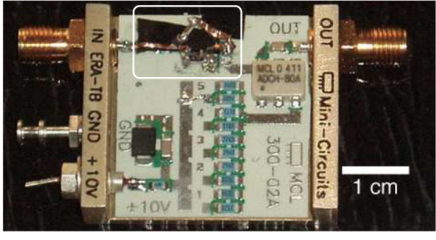
\includegraphics[width=\breite \columnwidth]{Fig1a}
         %       \caption{A gull}
   %             \label{fig:gull}
      %  \end{subfigure}
\subfloat[Bloque 1]{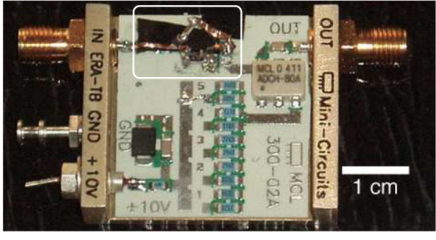
\includegraphics[width=\breite\linewidth]{Fig1a}}\\
\subfloat[Bloque 2]{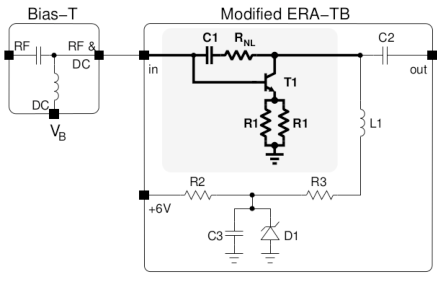
\includegraphics[width=\breite\linewidth]{Fig1b}}\\
\subfloat[Bloque 3]{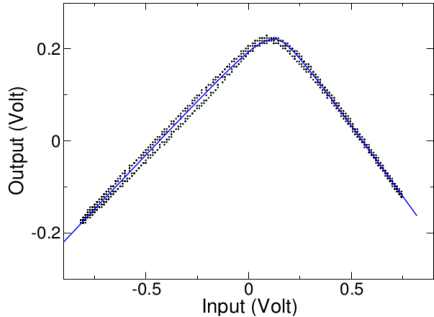
\includegraphics[width=\breite\linewidth]{Fig1c}}
\caption{Componentes del sistema propuesto: a) Tarjeta utilizada; b) Diagrama de circuito; c) Gráfica de respuesta
}
\label{fig:nonlinearity}
\end{figure}
%%%%%%%%%%%%%%%%%%%%%%%%%%%%%%%%%%%%%%%%%%%%%%%%%%%%
 
Si es necesario introducir una figura de mayor dimensión que ocupe las 2 columnas, es posible utilizar el ejemplo de la figura \ref{fig:setup}. 

\begin{figure*}
%\includegraphics*[width= \breite \columnwidth]{Fig2} 
%\includegraphics*[width= 1.6 \columnwidth]{Fig2} 
\subfloat[Imagen grandota Parte 1]{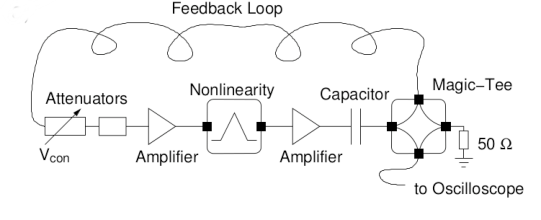
\includegraphics[width= \RelacionFiguradoscolumnas \linewidth]{Fig2a}}\\
\subfloat[Imagen grandota Parte 2]{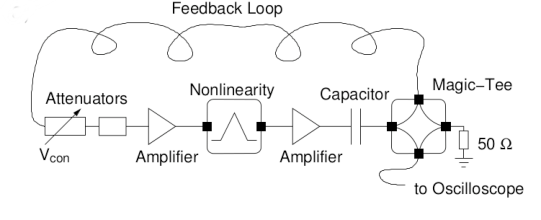
\includegraphics[width= \RelacionFiguradoscolumnas \linewidth]{Fig2a}}\\
\caption{El diagrama de la base de datos del sistema propuesto. (a). Diagrama detalladdo. (b). Diagrama específico de la tabla de alumnos, en donde se describen los principales campos. 
}
\label{fig:setup}
\end{figure*}
%%%%%%%%%%%%%%%%%%%%%%%%%%%%%%%%%%%%%%%%%%%%%%%%%%%%


\section{Resultados}

En esta sección es en donde debe ir las impresiones de pantalla que pongan en evidencia el sistema desarrollado. Además no basta con poner las pantallas del sistema, \textbf{SE DEBE EXPLICAR} el funcionamiento detallado de los componentes que aparecen en el mismo. 

En la figura \ref{fig:figura3}, se muestran diferentes pantallas del sistema implementado. En la figura \ref{fig:figura3}(a), se incluyen los principales controles de la interfaz de usuario diseñada. En la figura \ref{fig:figura3}(b), se muestra el resultado final de la aplicación ya en operación. 


%%%%%%%%%%%%%%%%%%%%%%%%%%%%%%%%%%%%%%%%%%%%%%%%%%%%
% FIGURE 3
%%%%%%%%%%%%%%%%%%%%%%%%%%%%%%%%%%%%%%%%%%%%%%%%%%%%
%
%
% 
\begin{figure}
\subfloat[Imagen grandota]{
\includegraphics[width=\breite\columnwidth]{CGUTP2}}\\
\subfloat[Imagen grandota]{
\includegraphics[width=\breite\columnwidth]{logo-web_2012-257x260}}\\
%\includegraphics*[width=\breite \columnwidth]{Fig3} 
\caption{Logotipos utilizados por las instancias educativas a nivel nacional. (a) Logotipo de la Coordinación de Universidades Tecnológicas y Politécnicas, con letras erdes muy feas por cierto. (b) Logotipo de la instutción alma máter de cualquier lecotr de este artículo}
\label{fig:figura3}
\end{figure}
%%%%%%%%%%%%%%%%%%%%%%%%%%%%%%%%%%%%%%%%%%%%%%%%%%%%




%%%%%%%%%%%%%%%%%%%%%%%%%%%%%%%%%%%%%%%%%%%%%%%%%%%%
% FIGURE 4
%%%%%%%%%%%%%%%%%%%%%%%%%%%%%%%%%%%%%%%%%%%%%%%%%%%%
%
%
En la figura \ref{fig:r2c_exp}, se muestran las funciones que pueden ser graficadas por el sistema. En la figura \ref{fig:r2c_exp}(a), se muestra la funcion $sin(x)$. De manera similar, en la figura \ref{fig:r2c_exp}(a) se muestra la función $cos(x)$.   

% 
\begin{figure}
%\includegraphics*[width=\breite \columnwidth]{Fig5} 
% PRIMERA FILA
\subfloat[Pos11\label{img11}]{
\includegraphics[width=0.3 \columnwidth]{UPV}}
\subfloat[Pos12\label{img12}]{
\includegraphics[width=0.3 \columnwidth]{CG}}
\subfloat[Pos13\label{img13}]{
\includegraphics[width=0.3 \columnwidth]{UPV}}
\\
% SEGUNDA FILA
\subfloat[Pos21]{
\includegraphics[width=0.3 \columnwidth]{UPV}}
\subfloat[Pos22]{
\includegraphics[width=0.3 \columnwidth]{CGUTP2}}
\subfloat[Pos23]{
\includegraphics[width=0.3 \columnwidth]{CGUTP2}}
\\
\subfloat[Pos31]{
\includegraphics[width=0.3 \columnwidth]{CGUTP2}}
\subfloat[Pos32]{
\includegraphics[width=0.3 \columnwidth]{UPV}}
\subfloat[Pos33]{
\includegraphics[width=0.3 \columnwidth]{CGUTP2}}
\\
\subfloat[Pos41]{
\includegraphics[width=0.3 \columnwidth]{CGUTP2}}
\subfloat[Pos42]{
\includegraphics[width=0.3 \columnwidth]{CGUTP2}}
\subfloat[Pos43]{
\includegraphics[width=0.3 \columnwidth]{UPV}}
\caption{Figura que demuestra como es posible incluir figuras con multiples subimagenes. En la figura \ref{img11}, el logotimo de la UPV. }
\label{fig:r2c_exp}
\end{figure}
%%%%%%%%%%%%%%%%%%%%%%%%%%%%%%%%%%%%%%%%%%%%%%%%%%%%


Para mostrar el funcionamiento de la aplicación se incluyen diversas pantallas de funcionamiento. En la figura \ref{fig:PNG}, se muestra la pantalla de login, en donde se muestran el cuadro para captura del usuario y el cuadro para capturar el password, además de un botón. En la figura \ref{fig:JPG}, se muestra la pantalla que aparece inmediatamente despues de que el usuario ingresa al sistema.

%%%%%%%%%%%%%%%%%%%%%%%%%%%%%%%%%%%%%%%%%%%%%%%%%%%%
% FIGURE PNG
%%%%%%%%%%%%%%%%%%%%%%%%%%%%%%%%%%%%%%%%%%%%%%%%%%%%
%
%
% 
\begin{figure}
\includegraphics*[width=\breite \columnwidth]{phd101212s} 
\caption{Ejemplo de inserción de una figura en formato PNG }
\label{fig:PNG}
\end{figure}
%%%%%%%%%%%%%%%%%%%%%%%%%%%%%%%%%%%%%%%%%%%%%%%%%%%%



%%%%%%%%%%%%%%%%%%%%%%%%%%%%%%%%%%%%%%%%%%%%%%%%%%%%
% FIGURE 1
%%%%%%%%%%%%%%%%%%%%%%%%%%%%%%%%%%%%%%%%%%%%%%%%%%%%
%
%
% 
\begin{figure}
\includegraphics*[width=\breite \columnwidth]{113114164} 
\caption{Ejemplo de inserción de una figura en formato JPG }
\label{fig:JPG}
\end{figure}
%%%%%%%%%%%%%%%%%%%%%%%%%%%%%%%%%%%%%%%%%%%%%%%%%%%%

En algunos casos es necesario desplegar información en tablas (según ustedes, nunca). Para esto es necesario utilizar ciertos comandos. \textit{En la tabla \ref{tabla1}, se muestra el listado del número de frames por segundo logrados con el programa implementado.} 

%\begin{table}[h!]  %% NO UTILIZAR NUNCA EL [h!]
\begin{table}
  \centering
  \caption{FPS obtenidos por el programa}
  \label{tab:table1}
  \begin{tabular}{l|c||r}
    Versión & FPS & FPS con mejor\\
    \hline
    a & 30 & 45\\
    b & 10 & 35\\
  \end{tabular}
  \label{tabla1}
\end{table}

En algunos casos, no es posible colocar el total de la información a dos columnas, por lo que se debe utilizar algo muy parecido a la figura \ref{fig:setup}. \textit{En la tabla \ref{tabla2}, se muestra el resultado del análisis del clima a lo largo de la semana en la que se desarrolló la aplicación, en Ciudad Victoria, Tamaulipas. Se puede notar que fue un clima muy agradable, lo que favoreció al logro del objetivo.}

\begin{table*}[h!]
  \centering
  \caption{Resumen climatológico de la semana durante la cual se llevo a cabo el estudio}
    \begin{tabular}{ | l | l | l | p{5cm} |}
    \hline
    Day & Min Temp & Max Temp & Summary \\ \hline
    Monday & 11C & 22C & A clear day with lots of sunshine.  
    However, the strong breeze will bring down the temperatures. \\ \hline
    Tuesday & 9C & 19C & Cloudy with rain, across many northern regions. Clear spells 
    across most of Scotland and Northern Ireland, 
    but rain reaching the far northwest. \\ \hline
    Wednesday & 10C & 21C & Rain will still linger for the morning. 
    Conditions will improve by early afternoon and continue 
    throughout the evening. \\
    \hline
    \end{tabular}
    \label{tabla2}
\end{table*}


\section{Conclusión}

En años anteriores, muchos dejan las conclusiones en negritas, prueba que nisiquiera leen lo que estan escribiendo simplemente copian y pegan y nisiquiera hacen un análisis. Los reto a volver a hacerlo. Pongo un ejemplo de dos conclusiones (una correcta y otra errónea).

\textbf{Conclusión Errónea: En este trabajo he aprendido a trabajar en equipo y a analizar la información de mejor manera. Además he tenido un crecimiento profesional, volvíendome un mejor ser humano, más humano y más sensible.... }

\textbf{Conclusión Correcta: En este trabajo se propone una solución a un problema X utilizando Y, Z o W cosa. Para logar se buscó en la computadora del profe juan para ver si había algun problema pareceido que me pudiera servir, se buscó en internet, se buscó en la plaza hidalgo. A partir de la información recopilada, se propuso un diseño nuevo, el cual fue implementado en tal computadora ....  Los resultados obtenidos ....}

\section*{Uso de referencias [Esta sección no es parte del informe]}

Se recomienda a los autores el uso de por lo menos 10 referencias, preferentemente balanceadas (esto es, 50\% originadas en páginas de internet y el otro 50\% originadas en libros especializados en la materia)

\addcontentsline{toc}{section}{Referencias} 
\printbibliography
%\balance



\end{document}













